%-----------------------------------------------------------------------------%
\chapter{\babLima}
%-----------------------------------------------------------------------------%
Bagian ini berisi hasil eksperimen terhadap Tensorflow Lite \textit{kernel} baru yang berjalan di GPU yang telah diimplementasikan menggunakan OpenCL. Pada akhir bagian ini diberikan analisis terhadap hasil eksperimen. Terdapat dua operasi yang diuji, yaitu perkalian matriks-matriks dan konvolusi matriks. Eksperimen dilakukan dengan cara memberikan ukuran masukan yang bervariasi terhadap operasi-operasi tersebut. Untuk masing-masing operasi, penulis membandingkan kecepatan dari \textit{OpenCL kernel}, \textit{naive kernel}, dan \textit{optimized kernel}. Kecepatan dari \textit{kernel} diukur menggunakan \textit{wall-clock time}. Penulis menghitung rata-rata kecepatan dari 10 kali eksekusi \textit{kernel} dan juga menghitung standar deviasinya. Satuan yang digunakan untuk mengukur waktu adalah \textit{milisecond}. Eksperimen ini dilakukan pada perangkat Android dengan spesifikasi berikut.

\begin{enumerate}
	\item CPU : Snapdragon 435, 8x ARM Cortex-A53 @ 1.40Ghz
	\item GPU : Adreno 505, OpenCL 2.0 supported
	\item RAM : 3GB
\end{enumerate}

%-----------------------------------------------------------------------------%
\section{Eksperimen Terhadap \textit{Kernel} Operasi Perkalian Matriks-Matriks }
%-----------------------------------------------------------------------------%
Eksperimen ini bertujuan untuk menguji dan membandingkan kecepatan tiga jenis Tensorflow Lite \textit{kernel} untuk operasi perkalian matriks-matriks. Pada eksperimen ini digunakan ukuran yang sama untuk dua matriks masukan dan juga matriks keluaran. Terdapat lima variasi ukuran $panjang \times lebar$ matriks yang diberikan, yaitu $64 \times 64$, $128 \times 128$, $256 \times 256$, $512 \times 512$, dan $1024 \times 1024$. Dengan demikian, akan terlihat \textit{kernel} mana saja yang unggul dalam komputasi matriks kecil dan \textit{kernel} mana saja yang unggul dalam komputasi matriks besar. Selain itu pada eksperimen ini juga akan terlihat bagaimana persiapan OpenCL berpengaruh terhadap kecepatan Tensorflow Lite \textit{kernel} untuk operasi perkalian matriks-matriks yang diimplementasikan menggunakan OpenCL. Akan diketahui \textit{bottleneck} dari OpenCL pada matriks besar dan matriks kecil. 

Hasil eksperimen terhadap kecepatan dari tiga jenis \textit{kernel} dapat dilihat pada \tab~\ref{tab:matmatmulspeed}. Nilai-nilai dari tabel tersebut dalah rata-rata (dalam \textit{milisecond}) dari 10 kali eksekusi \textit{kernel}. Standar deviasi dari 10 eksekusi tersebut dapat dilihat pada \tab~\ref{tab:matmatmuldev}. Secara visual, perbandingan kecepatan antara ketiga jenis \textit{kernel} dapat dilihat pada \pic~\ref{fig:matmatmul}. 

\begin{table}
	\centering
	\caption{Hasil eksperimen terhadap Tensorflow Lite \textit{kernel} untuk operasi perkalian matriks-matriks. Waktu dihitung menggunakan satuan detik dengan melakukan rata-rata dari 10 kali \textit{run}. Penyalinan data tidak dihitung untuk menentukan kecepatan.}
	\label{tab:matmatmulspeed}
	\begin{tabular}{| R{2cm} | R{2cm} | R{2cm} | R{2cm} | R{2cm} |}
		\hline
		\textbf{Matrix Sizes} & \textbf{Naive Kernel} & \textbf{Optimized Kernel} & \textbf{OpenCL Kernel} & \textbf{OpenCL + Setup} \\
		\hline
		64x64 & 4.3596 & 1.1243 & 1.5501 & 7.6569
		\\
		\hline
		128x128 & 33.9033 & 7.7470 & 2.3841 & 8.6730
		\\
		\hline
		256x256 & 205.9833 & 62.4273 & 14.2164 & 21.7435
		\\
		\hline
		512x512 & 1193.9166 & 373.4296 & 107.3510 & 116.6284
		\\
		\hline
		1024x1024 & 9518.9719 & 3507.8444 & 824.9642 & 848.4501
		\\
		\hline
	\end{tabular}
\end{table}

\begin{table}
	\centering
	\caption{Hasil eksperimen terhadap empat kernel operasi perkalian matriks-vektor. Waktu dihitung menggunakan satuan detik dengan melakukan rata-rata dari 10 kali \textit{run}. Penyalinan data tidak dihitung untuk menentukan kecepatan.}
	\label{tab:matmatmuldev}
	\begin{tabular}{| R{2cm} | R{2cm} | R{2cm} | R{2cm} | R{2cm} |}
		\hline
		\textbf{Matrix Sizes} & \textbf{Naive Kernel} & \textbf{Optimized Kernel} & \textbf{OpenCL Kernel} & \textbf{OpenCL + Setup} \\
		\hline
		64x64 & 0.0958 & 0.1270 & 0.0726 & 0.7545
		\\
		\hline
		128x128 & 0.4717 & 0.7324 & 0.0504 & 1.0877
		\\
		\hline
		256x256 & 4.5170 & 1.3869 & 0.0912 & 0.9902
		\\
		\hline
		512x512 & 1.8006 & 3.3557 & 0.1832 & 0.8476
		\\
		\hline
		1024x1024 & 3.1632 & 10.8558 & 0.1265 & 0.9315
		\\
		\hline
	\end{tabular}
\end{table}

\begin{figure}
	\centering
	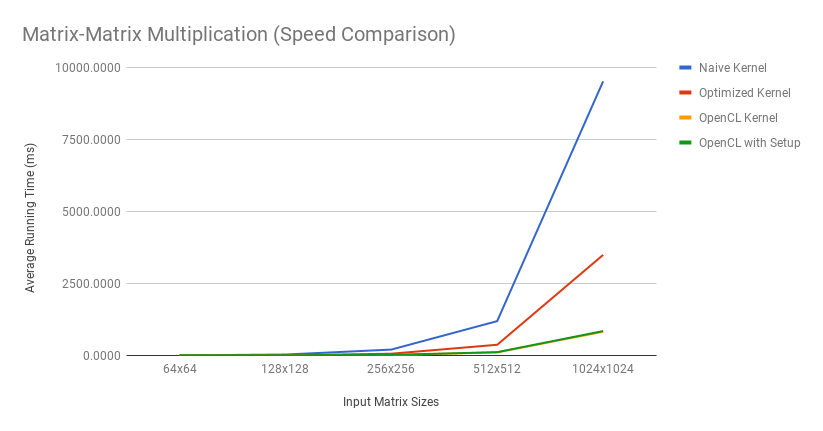
\includegraphics[width=0.50\textwidth]
	{pics/matmatmul.png}
	\caption{Perbandingan kecepatan empat kernel pada operasi perkalian matriks-vektor tanpa memperhitungkan proses penyalinan data antara CPU dan GPU (ukuran 128x128 hingga 1024x1024).}
	\label{fig:matmatmul}
\end{figure}

Dari hasil eksperimen di atas dapat dilihat bahwa Tensorflow Lite \textit{kernel} untuk operasi perkalian matriks-matriks yang berjalan di GPU melalui OpenCL memiliki performa yang paling baik, terutama untuk matriks berukuran besar. Ketika hanya mempertimbangkan kecepatan komputasi OpenCL \textit{kernel} (tanpa menghitung persiapan), OpenCL \textit{kernel} memiliki performa yang lebih baik dari dua \textit{kernel} lain saat ukuran matriks $128 \times 128$ atau lebih besar. Sementara itu ketika persiapan OpenCL dimasukkan ke dalam penghitungan, OpenCL \textit{kernel} baru mencapai performa terbaik ketika ukuran matriks $256 \times 256$ atau lebih besar.

\section{Eksperimen Terhadap \textit{Kernel} Operasi Konvolusi Matriks }
%-----------------------------------------------------------------------------%
Eksperimen ini bertujuan untuk menguji dan membandingkan kecepatan tiga jenis Tensorflow Lite \textit{kernel} untuk operasi konvolusi matriks. Pada eksperimen ini digunakan beberapa jenis ukuran matriks-matriks masukan dan matriks keluaran. Untuk operasi ini penulis membagi eksperimen ke dalam tiga kasus uji, antara lain kasus ketika ukuran $panjang \times lebar$ bervariasi, kasus ketika ukuran $panjang \times lebar$ bervariasi, dan kasus ketika ukuran $panjang \times lebar$ bervariasi. Pada eksperimen ini akan terlihat \textit{kernel} mana saja yang unggul dalam berbagai kasus yang diberikan. Selain itu juga akan terlihat bagaimana persiapan OpenCL berpengaruh terhadap kecepatan Tensorflow Lite \textit{kernel} untuk operasi konvolusi yang menggunakan OpenCL. Akan diketahui \textit{bottleneck} dari OpenCL pada berbagai kasus uji.

\subsection{Eksperimen Konvolusi dengan Panjang dan Lebar \textit{Image} yang Bervariasi}
Pada eksperimen ini, diberikan matriks \textit{image} dengan panjang dan lebar yang bervariasi sehingga dapat diketahui bagaimana besar kecilnya ukuran panjang dan lebar \textit{image} mempengaruhi kecepatan dari tiga jenis \textit{kernel}. Spesifikasi ukuran dari matriks image dan filter yang digunakan dapat dilihat pada \tab~\ref{tab:imagefilterspec1}. Terdapat lima variasi ukuran $panjang \times lebar$ matriks \textit{image} yang diberikan, yaitu $32 \times 32$, $64 \times 64$, $128 \times 128$, $256 \times 256$, dan $512 \times 512$. Dalam OpenCL, panjang dan lebar dari \textit{image} terkait dengan panjang dan lebar dari \textit{work-space} yang digunakan dalam eksekusi OpenCL \textit{kernel}. Hal ini telah dijelaskan pada BAB III.

\begin{table}
	\centering
	\caption{Spesifikasi ukuran matriks \textit{image} dan \textit{filter} yang diujikan untuk operasi konvolusi pada kasus panjang dan lebar \textit{image} yang bervariasi.}
	\label{tab:imagefilterspec1}
	\begin{tabular}{| R{2cm} | R{2cm} | R{2cm} | R{2cm} | R{2cm} |}
		\hline
		\textbf{Matrix} & \textbf{Channel} & \textbf{Height} & \textbf{Width} & \textbf{Batch} 
		\\
		\hline
		Image & 4 & varying & varying & 1
		\\
		\hline
		Filter & 4 & 5 & 5 & 4
		\\
		\hline
	\end{tabular}
\end{table}

Hasil eksperimen terhadap kecepatan dari tiga jenis \textit{kernel} pada kasus bervariasinya panjang dan lebar \textit{image} ini dapat dilihat pada \tab~\ref{tab:convvarhwspeed}. Nilai-nilai dari tabel tersebut dalah rata-rata (dalam \textit{milisecond}) dari 10 kali eksekusi \textit{kernel}. Standar deviasi dari 10 eksekusi tersebut dapat dilihat pada \tab~\ref{tab:convvarhwdev}. Secara visual, perbandingan kecepatan antara ketiga jenis \textit{kernel} dapat dilihat pada \pic~\ref{fig:convvarhw}.

\begin{table}
	\centering
	\caption{Hasil eksperimen terhadap empat kernel operasi perkalian matriks-vektor. Waktu dihitung menggunakan satuan detik dengan melakukan rata-rata dari 10 kali \textit{run}. Penyalinan data juga dihitung untuk menentukan kecepatan.}
	\label{tab:convvarhwspeed}
	\begin{tabular}{| R{2cm} | R{2cm} | R{2cm} | R{2cm} | R{2cm} |}
		\hline
		\textbf{Image HxW} & \textbf{Naive Kernel} & \textbf{Optimized Kernel} & \textbf{OpenCL Kernel} & \textbf{OpenCL + Setup} 
		\\
		\hline
		32x32 & 6.6511 & 4.7852 & 1.5196 & 6.1364
		\\
		\hline
		64x64 & 31.3152 & 13.4992 & 1.8377 & 7.9563
		\\
		\hline
		128x128 & 113.8935 & 43.4996 & 5.5047 & 13.1798
		\\
		\hline
		256x256 & 366.5030 & 122.3684 & 20.1672 & 31.9092
		\\
		\hline
		512x512 & 1283.9716 & 401.0434 & 79.5439 & 111.8054
		\\
		\hline
	\end{tabular}
\end{table}

\begin{table}
	\centering
	\caption{Hasil eksperimen terhadap empat kernel operasi perkalian matriks-vektor. Waktu dihitung menggunakan satuan detik dengan melakukan rata-rata dari 10 kali \textit{run}. Penyalinan data juga dihitung untuk menentukan kecepatan.}
	\label{tab:convvarhwdev}
	\begin{tabular}{| R{2cm} | R{2cm} | R{2cm} | R{2cm} | R{2cm} |}
		\hline
		\textbf{Image HxW} & \textbf{Naive Kernel} & \textbf{Optimized Kernel} & \textbf{OpenCL Kernel} & \textbf{OpenCL + Setup} 
		\\
		\hline
		32x32 & 0.4444 & 0.9186 & 0.1311 & 0.6996
		\\
		\hline
		64x64 & 0.9173 & 2.5479 & 0.0799 & 1.3398
		\\
		\hline
		128x128 & 6.9582 & 9.9099 & 0.2741 & 1.5212
		\\
		\hline
		256x256 & 9.9799 & 4.9044 & 0.3141 & 1.8619
		\\
		\hline
		512x512 & 10.8159 & 3.3544 & 0.1262 & 1.7571
		\\
		\hline
	\end{tabular}
\end{table}

\begin{figure}
	\centering
	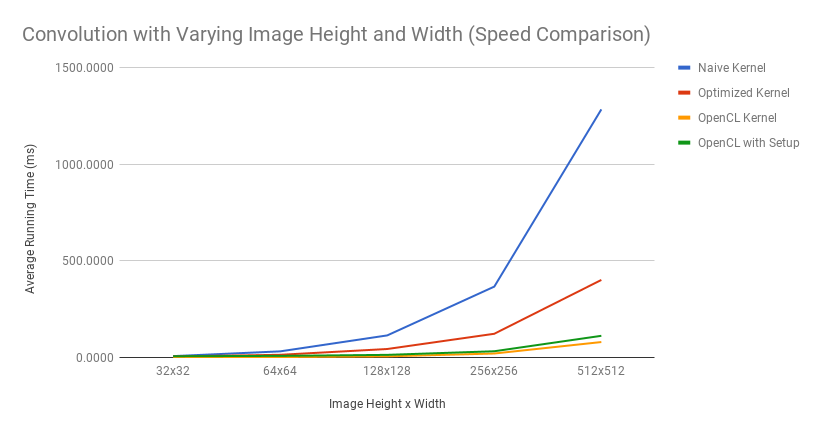
\includegraphics[width=0.50\textwidth]
	{pics/convvarhw.png}
	\caption{Perbandingan kecepatan empat kernel pada operasi perkalian matriks-vektor dengan memperhitungkan proses penyalinan data antara CPU dan GPU (ukuran 128x128 hingga 1024x1024).}
	\label{fig:convvarhw}
\end{figure}

Dari hasil eksperimen di atas dapat dilihat bahwa Tensorflow Lite \textit{kernel} untuk operasi konvolusi yang berjalan di GPU melalui OpenCL memiliki performa yang paling baik. Ketika hanya mempertimbangkan kecepatan komputasi OpenCL \textit{kernel} (tanpa menghitung persiapan), OpenCL \textit{kernel} memiliki performa yang lebih baik dari dua \textit{kernel} lain pada semua variasi ukuran matriks yang diuji. Sementara itu ketika persiapan OpenCL dimasukkan ke dalam penghitungan, OpenCL \textit{kernel} baru mencapai performa terbaik saat $panjang \times lebar$ dari \textit{image} berukuran $64 \times 64$ atau lebih besar.

\subsection{Eksperimen Konvolusi dengan Banyak Kanal \textit{Image} yang Bervariasi}
Pada eksperimen ini, diberikan matriks \textit{image} dengan banyaknya kanal yang bervariasi sehingga dapat diketahui bagaimana banyak sedikitnya kanal dari \textit{image} mempengaruhi kecepatan dari tiga jenis \textit{kernel}. Spesifikasi ukuran dari matriks image dan filter yang digunakan dapat dilihat pada \tab~\ref{tab:imagefilterspec2}. Terdapat lima variasi banyaknya kanal matriks \textit{image} yang diberikan, yaitu $64$, $128$, $256$, $512$, dan $1024$. Dalam OpenCL, banyaknya kanal dari \textit{image} terkait dengan banyaknya iterasi ketika melakukan konvolusi pada setiap \textit{work-item}. Hal ini telah dijelaskan pada BAB III. Semakin besar ukuran kanal dari \textit{image}, semakin besar pula beban komputasi yang dikerjakan oleh suatu \textit{work-item}.

\begin{table}
	\centering
	\caption{Spesifikasi ukuran matriks \textit{image} dan \textit{filter} yang diujikan untuk operasi konvolusi pada kasus banyaknya kanal dari \textit{image} yang bervariasi.}
	\label{tab:imagefilterspec2}
	\begin{tabular}{| R{2cm} | R{2cm} | R{2cm} | R{2cm} | R{2cm} |}
		\hline
		\textbf{Matrix} & \textbf{Channel} & \textbf{Height} & \textbf{Width} & \textbf{Batch} 
		\\
		\hline
		Image & varying & 16 & 16 & 1
		\\
		\hline
		Filter & varying & 5 & 5 & 4
		\\
		\hline
	\end{tabular}
\end{table}

Hasil eksperimen terhadap kecepatan dari tiga jenis \textit{kernel} dalam kasus bervariasinya banyak kanal \textit{image} ini dapat dilihat pada \tab~\ref{tab:convvarchnspeed}. Nilai-nilai dari tabel tersebut dalah rata-rata (dalam \textit{milisecond}) dari 10 kali eksekusi \textit{kernel}. Standar deviasi dari 10 eksekusi tersebut dapat dilihat pada \tab~\ref{tab:convvarchndev}. Secara visual, perbandingan kecepatan antara ketiga jenis \textit{kernel} dapat dilihat pada \pic~\ref{fig:convvarchn}.

\begin{table}
	\centering
	\caption{Hasil eksperimen terhadap empat kernel operasi perkalian matriks-vektor. Waktu dihitung menggunakan satuan detik dengan melakukan rata-rata dari 10 kali \textit{run}. Penyalinan data juga dihitung untuk menentukan kecepatan.}
	\label{tab:convvarchnspeed}
	\begin{tabular}{| R{2cm} | R{2cm} | R{2cm} | R{2cm} | R{2cm} |}
		\hline
		\textbf{Image Channel} & \textbf{Naive Kernel} & \textbf{Optimized Kernel} & \textbf{OpenCL Kernel} & \textbf{OpenCL + Setup} 
		\\
		\hline
		64 & 12.4833 & 12.8914 & 1.6086 & 9.1080
		\\
		\hline
		128 & 24.3573 & 24.1618 & 2.8356 & 9.9595
		\\
		\hline
		256 & 52.3216 & 51.8085 & 5.0332 & 13.4032
		\\
		\hline
		512 & 85.7740 & 92.0345 & 8.6298 & 15.9954
		\\
		\hline
		1024 & 152.1905 & 165.9758 & 19.0146 & 26.8229
		\\
		\hline
	\end{tabular}
\end{table}

\begin{table}
	\centering
	\caption{Hasil eksperimen terhadap empat kernel operasi perkalian matriks-vektor. Waktu dihitung menggunakan satuan detik dengan melakukan rata-rata dari 10 kali \textit{run}. Penyalinan data juga dihitung untuk menentukan kecepatan.}
	\label{tab:convvarchndev}
	\begin{tabular}{| R{2cm} | R{2cm} | R{2cm} | R{2cm} | R{2cm} |}
		\hline
		\textbf{Image Channel} & \textbf{Naive Kernel} & \textbf{Optimized Kernel} & \textbf{OpenCL Kernel} & \textbf{OpenCL + Setup} 
		\\
		\hline
		64 & 1.2069 & 1.0923 & 0.0874 & 1.1450
		\\
		\hline
		128 & 2.2827 & 1.9532 & 0.3127 & 1.4827
		\\
		\hline
		256 & 1.8923 & 4.9887 & 0.5981 & 1.8302
		\\
		\hline
		512 & 6.2608 & 3.8101 & 0.1258 & 0.8930
		\\
		\hline
		1024 & 2.0152 & 9.3311 & 0.2196 & 0.9503
		\\
		\hline
	\end{tabular}
\end{table}

\begin{figure}
	\centering
	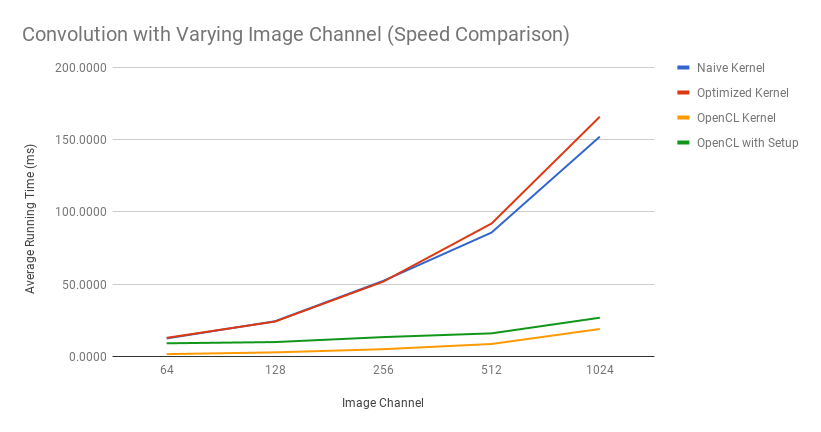
\includegraphics[width=0.50\textwidth]
	{pics/convvarchn.png}
	\caption{Perbandingan kecepatan empat kernel pada operasi perkalian matriks-vektor dengan memperhitungkan proses penyalinan data antara CPU dan GPU (ukuran 128x128 hingga 1024x1024).}
	\label{fig:convvarchn}
\end{figure}

Dari hasil eksperimen di atas dapat dilihat bahwa Tensorflow Lite \textit{kernel} untuk operasi konvolusi yang berjalan di GPU melalui OpenCL memiliki performa yang paling baik. Ketika waktu untuk persiapan OpenCL diperhitungkan maupun ketika tidak diperhitungkan, OpenCL \textit{kernel} memiliki performa yang lebih baik dari dua \textit{kernel} lainnya pada semua variasi ukuran matriks yang diuji.

\subsection{Eksperimen Konvolusi dengan Banyak \textit{Batch} dan Kanal \textit{Output} yang Bervariasi}
Pada eksperimen ini, diberikan matriks \textit{image} dan \textit{filter} dengan \textit{batch} yang bervariasi. Banyaknya \textit{batch} dari \textit{image} sama dengan banyaknya \textit{batch} dari \textit{output}, sedangkan banyaknya \textit{batch} dari \textit{filter} sama dengan banyaknya kanal dari \textit{output}. Pada eksperimen ini ingin diketahui bagaimana banyak sedikitnya \textit{batch} dan kanal dari \textit{output} mempengaruhi kecepatan tiga jenis kernel \textit{kernel}. Spesifikasi ukuran dari matriks image dan filter yang digunakan dapat dilihat pada \tab~\ref{tab:imagefilterspec3}. Terdapat lima variasi ukuran $panjang \times lebar$ matriks \textit{image} yang diberikan, yaitu $8 \times 8$, $16 \times 16$, $32 \times 32$, $64 \times 64$, dan $128 \times 128$. Dalam OpenCL, banyaknya \textit{batch} dan kanal dari matriks \textit{output} terkait dengan lebar dan panjang dari \textit{work-space} yang digunakan dalam eksekusi OpenCL \textit{kernel}. Hal ini telah dijelaskan pada BAB III.

\begin{table}
	\centering
	\caption{Spesifikasi ukuran matriks \textit{image} dan \textit{filter} yang diujikan untuk operasi konvolusi pada kasus banyaknya \textit{batch} dan \textit{kanal} dari \textit{output} yang bervariasi.}
	\label{tab:imagefilterspec3}
	\begin{tabular}{| R{2cm} | R{2cm} | R{2cm} | R{2cm} | R{2cm} |}
		\hline
		\textbf{Matrix} & \textbf{Channel} & \textbf{Height} & \textbf{Width} & \textbf{Batch} 
		\\
		\hline
		Image & 4 & 16 & 16 & varying
		\\
		\hline
		Filter & 4 & 5 & 5 & varying
		\\
		\hline
	\end{tabular}
\end{table}

Hasil eksperimen terhadap kecepatan dari tiga jenis \textit{kernel} pada kasus bervariasinya banyak \textit{batch} dan kanal \textit{output} ini dapat dilihat pada \tab~\ref{tab:convvarbchnspeed}. Nilai-nilai dari tabel tersebut dalah rata-rata (dalam \textit{milisecond}) dari 10 kali eksekusi \textit{kernel}. Standar deviasi dari 10 eksekusi tersebut dapat dilihat pada \tab~\ref{tab:convvarbchndev}. Secara visual, perbandingan kecepatan antara ketiga jenis \textit{kernel} dapat dilihat pada \pic~\ref{fig:convvarbchn}.

\begin{table}
	\centering
	\caption{Hasil eksperimen terhadap empat kernel operasi perkalian matriks-vektor. Waktu dihitung menggunakan satuan detik dengan melakukan rata-rata dari 10 kali \textit{run}. Penyalinan data juga dihitung untuk menentukan kecepatan.}
	\label{tab:convvarbchnspeed}
	\begin{tabular}{| R{2cm} | R{2cm} | R{2cm} | R{2cm} | R{2cm} |}
		\hline
		\textbf{Output BxC} & \textbf{Naive Kernel} & \textbf{Optimized Kernel} & \textbf{OpenCL Kernel} & \textbf{OpenCL + Setup} 
		\\
		\hline
		8x8 & 21.3206 & 6.8149 & 1.7034 & 9.6239
		\\
		\hline
		16x16 & 77.6343 & 11.5020 & 4.5229 & 12.9872
		\\
		\hline
		32x32 & 241.5599 & 20.3202 & 15.9239 & 24.1819
		\\
		\hline
		64x64 & 756.2591 & 44.4415 & 61.0587 & 75.0377
		\\
		\hline
		128x128 & 2847.1164 & 106.8449 & 236.1338 & 262.0281
		\\
		\hline
	\end{tabular}
\end{table}

\begin{table}
	\centering
	\caption{Hasil eksperimen terhadap empat kernel operasi perkalian matriks-vektor. Waktu dihitung menggunakan satuan detik dengan melakukan rata-rata dari 10 kali \textit{run}. Penyalinan data juga dihitung untuk menentukan kecepatan.}
	\label{tab:convvarbchndev}
	\begin{tabular}{| R{2cm} | R{2cm} | R{2cm} | R{2cm} | R{2cm} |}
		\hline
		\textbf{Output BxC} & \textbf{Naive Kernel} & \textbf{Optimized Kernel} & \textbf{OpenCL Kernel} & \textbf{OpenCL + Setup} 
		\\
		\hline
		8x8 & 2.4153 & 0.6333 & 0.1556 & 1.5570
		\\
		\hline
		16x16 & 4.3455 & 1.6288 & 0.2239 & 1.4405
		\\
		\hline
		32x32 & 7.2629 & 1.5248 & 0.1507 & 1.0567
		\\
		\hline
		64x64 & 3.0043 & 1.2937 & 0.0650 & 2.5150
		\\
		\hline
		128x128 & 8.1991 & 7.3458 & 0.6611 & 10.9892
		\\
		\hline
	\end{tabular}
\end{table}

\begin{figure}
	\centering
	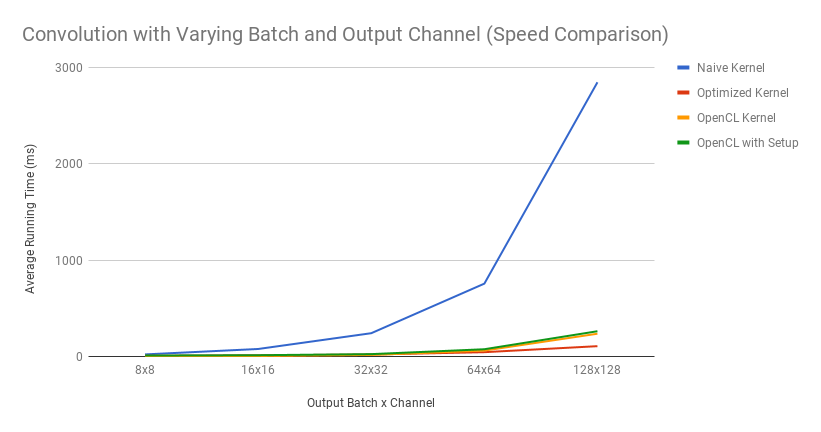
\includegraphics[width=0.50\textwidth]
	{pics/convvarbchn.png}
	\caption{Perbandingan kecepatan empat kernel pada operasi perkalian matriks-vektor dengan memperhitungkan proses penyalinan data antara CPU dan GPU (ukuran 128x128 hingga 1024x1024).}
	\label{fig:convvarbchn}
\end{figure}

Dari hasil eksperimen di atas dapat dilihat bahwa Tensorflow Lite \textit{optimized kernel} yang berjalan di CPU memiliki performa yang paling baik ketika ukuran matriks \textit{output} semakin besar. \textit{Optimized kernel} mampu mengungguli performa OpenCL \textit{kernel} tanpa persiapan ketika $batch \times kanal$ dari \textit{output} berukuran $64 \times 64$ atau lebih besar. \textit{Optimized kernel} juga mampu mengungguli performa OpenCL \textit{kernel} pada semua variasi ukuran matriks \textit{output} yang diuji ketika persiapan OpenCL diperhitungkan.

%-----------------------------------------------------------------------------%
\section{Analisis }
%-----------------------------------------------------------------------------%
